\documentclass{article}
\usepackage{listings}
\usepackage{color}
\usepackage[margin=1in]{geometry} % Set margins to 1 inch
\usepackage{graphicx} % Allows including images
\usepackage{float} % Allows for precise placement of figures
\usepackage{amsmath} % Allows for math equations
\usepackage{siunitx} % Allows for SI units
\usepackage{placeins} % Makes sure images are in their respective sections by \FloatBarrier


% Define code listing style
\lstset{
    language=Python,
    basicstyle=\small\ttfamily,
    keywordstyle=\color{blue},
    stringstyle=\color{red},
    commentstyle=\color{green},
    numbers=left,
    numberstyle=\tiny,
    numbersep=5pt,
    breaklines=true,
    showstringspaces=false,
    frame=tb,
    captionpos=b
}

\title{Random Number Generator using Shift Registers and XOR Gates}
\author{Anirudh Saikrishnan \\ CS22BTECH11004}
\date{\today}

\begin{document}

\maketitle

\section{Introduction}

Random number generators (RNGs) are essential in various computational applications that require randomness, such as simulations, cryptography, and gaming. In this report, we will discuss the concept of creating a random number generator using shift registers and XOR gates.

\section{Components}
\begin{enumerate}    
    \item Breadboard
    \item Seven Segment Display : Common Anode
    \item Seven Segment Display Decoder [7447]
    \item FlipFlop [7474] x2
    \item XOR gate [7486]
    \item 555 IC
    \item Resistors [10M$\Omega$, 1K$\omega$ x2]
    \item Capacitors [47nF,470nF]
    \item USB micro B breakout board
    \item Jumper wires
\end{enumerate}

\begin{figure}[ht]
        \centering
        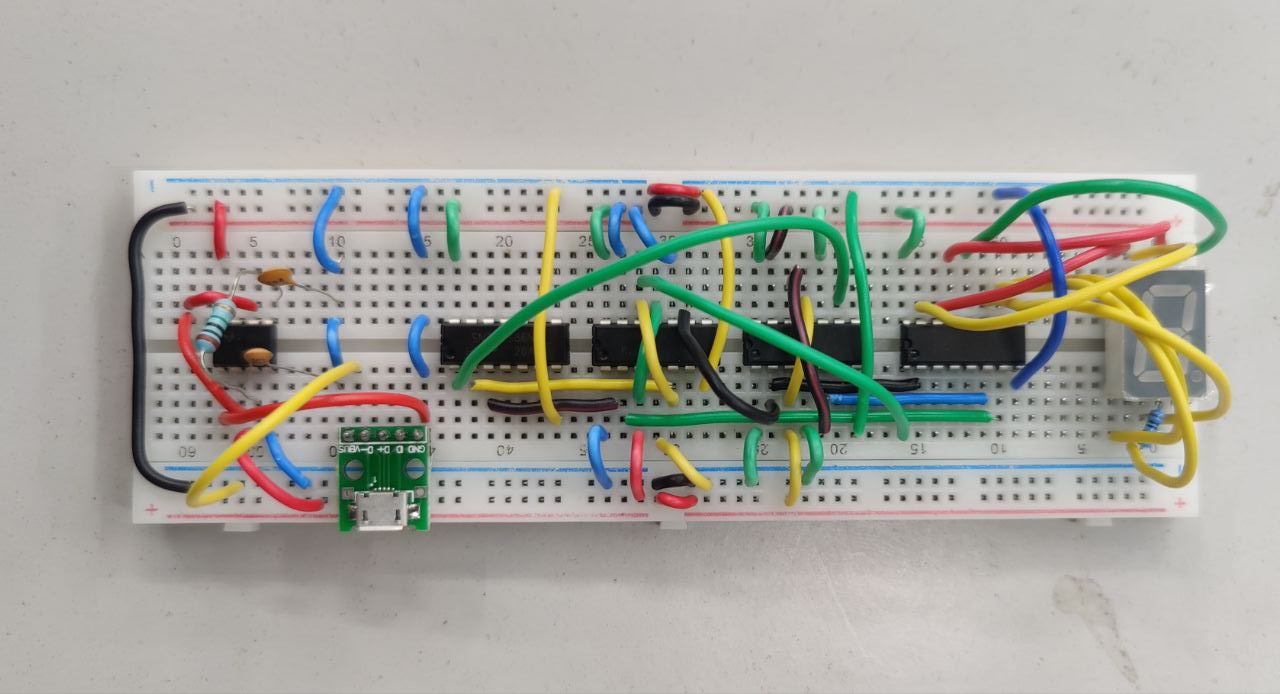
\includegraphics[width=1\linewidth]{CircuitBoard.jpeg}
        \caption{Circuit Board}
        \label{fig:view}
\end{figure}


\section{Shift Registers}

Shift registers are sequential logic circuits composed of flip-flops connected in a chain. They can store and shift binary data based on a clock signal. The data stored in the registers is shifted from one flip-flop to another, allowing for sequential processing.

\section{XOR Gates}

XOR gates are digital logic gates that produce an output of "1" if the number of "1" inputs is odd, and "0" otherwise. XOR gates are commonly used in various applications, including binary addition, error detection, and randomness generation.

\section{Creating a Random Number Generator}

To create a random number generator using shift registers and XOR gates, we can utilize the concept of feedback shift registers (FSRs) with XOR operations. FSRs generate a sequence of pseudo-random numbers based on the feedback of selected flip-flops through XOR gates.

\subsection{Algorithm}

The following algorithm describes the steps to create a random number generator using shift registers and XOR gates:

\begin{enumerate}
    \item Initialize the shift register with an initial seed value.
    \item Generate a clock signal.
    \item Shift the register contents one bit to the right.
    \item Compute the next bit based on the XOR operation of selected flip-flop outputs.
    \item Append the computed bit to the leftmost side of the register.
    \item Repeat steps 3-5 to generate the next random number.
\end{enumerate}

\section{Conclusion}

In this report, we discussed the concept of creating a random number generator using shift registers and XOR gates. We explained the working principle of shift registers and XOR gates and described the algorithm to generate random numbers. We also provided a Python implementation as an example. By utilizing feedback shift registers with XOR operations, we can generate pseudo-random numbers efficiently.

Random number generators are widely used in various applications, and understanding the underlying mechanisms can help in designing and implementing robust randomness generation techniques.

\section{Block Diagram}
\begin{figure}[ht]
        \centering
        \includegraphics[width=0.8\linewidth]{BlockDiagram.jpeg}
        \caption{Block Diagram}
        \label{fig:view}
\end{figure}


\end{document}

